%%%%%%%%%%%%%%%%%%%% author.tex %%%%%%%%%%%%%%%%%%%%%%%%%%%%%%%%%%%
%
% sample root file for your "contribution" to a contributed volume
%
% Use this file as a template for your own input.
%
%%%%%%%%%%%%%%%%%%%% author.tex %%%%%%%%%%%%%%%%%%%%%%%%%%%%%%%%%%%


% RECOMMENDED %%%%%%%%%%%%%%%%%%%%%%%%%%%%%%%%%%%%%%%%%%%%%%%%%%%
\documentclass{svmult}

% Choose options for [] as required from the list in the Reference Guide

\usepackage{mathptmx} 	% selects Times Roman as basic font
\usepackage{helvet} 		% selects Helvetica as sans-serif font
\usepackage{courier} 		% selects Courier as typewriter font
\usepackage{type1cm} 		% activate if the above 3 fonts are
								% not available on your system

\usepackage{makeidx} 		% allows index generation
\usepackage{graphicx} 	% standard LaTeX graphics tool

% when including figure files
\usepackage{multicol} 						% used for the two-column index
\usepackage[bottom]{footmisc} 			% places footnotes at page bottom
\usepackage{amsmath,amssymb,epsfig}
\usepackage{epstopdf}
\bibliographystyle{spmpsci}

% See the list of further useful packages in the Reference Guide

\makeindex 	% used for the subject index
				% please use the style svind.ist with
				% your makeindex program

% RECOMMENDED %%%%%%%%%%%%%%%%%%%%%%%%%%%%%%%%%%%%%%%%%%%%%%%%%%%

% Use the package "url.sty" to avoid problems with special characters used in your e-mail or web address
\begin{document}
\title*{Gaze-based control of robot-swarm using electroencephalography} % Fix!

% Use \titlerunning{Short Title} for an abbreviated version of your contribution title if the original one is too long

\author{Luca Mondada$^1$, Mohammad Ehsanul Karim$^2$, and Francesco Mondada$^2$}
\authorrunning{L Mondada, M E Karim and F Mondada}

% Use \authorrunning{Short Title} for an abbreviated version of your contribution title if the original one is too long

\institute{$^1$Department of Physics, Swiss Federal Institute of Technology ETHZ, Z\"urich, Switzerland, \email{Email address} \\
$^2$Laboratoire de Syst\`emes Robotiques, Ecole Polytechnique F\'ed\'erale de Lausanne, Lausanne, Switzerland, \email{Email address}} % Fix!

\maketitle

\abstract{Search and rescue, autonomous construction, and many other semiautonomous and distributed robotics application can benefit from an efficient human control over a robot-swarm. To-date most of the interactive swarm control relies on gesture and speech recognition based techniques. However such techniques are not quite intuitive in establishing connection between the human-user and a single robot in the swarm. This study proposes a new methodology to approach this problem of robot selection; we use electroencephalography (EEG) signals to select the robot the user is physically looking at. This is achieved by analyzing the steady-state visually evoked potential (SSVEP), a repeatable neural response to a regularly blinking visual stimulus that varies predictively based on the blinking frequency. In our experiments, the LED on the robots blinked at different frequencies and the user SSVEP signal was analyzed to detect and select the robot. This study systematically investigates several factors that directly impacts the efficiency of the system in the specific case of a human-swarm interaction; in particular, we study two algorithms and the various associated tuning parameters: distance between the robot and the user, the LED color, and LED blink frequency. Finally based on the studies, we propose a methodology and critically analyze it based its performance on 10 subjects controlling physical robots. Our results show that despite the numerous artifacts, it is possible to guarantee on average, a recognition rate of 75\% at any time after the first 4 seconds of EEG data acquisition.}

\keywords{human-swarm interactions, human-robot interaction, EEG, SSVEP, Emotiv EPOC}

\section{Introduction}
\label{sec:introduction}
Distributed multi-robot systems have extremely promising applications; for example: search for rescue, environmental monitoring, autonomous construction or geographical mapping. The topic has been extensively studied under various names: swarm robotics \cite{brambilla2013}, collective robotics \cite{kernbach2013handbook}, or distributed robotics \cite{martinoli2012distributed}. To-date researches and engineers have struggled in designing scalable \cite{rubenstein2012kilobot}, robust \cite{winfield2006safety}, efficient (compared to single robot) \cite{Bonani2012} and affordable distributed multi-robot systems \cite{rubenstein2014programmable}. In addition to the autonomous control strategies, there are multiple challenges from the human-robot interaction (HRI) point of view. Although many single-robot control interfaces have shown interesting results, efficiently controlling a robotic swarm is still a state-of-the-art problem.\\
\\
One of the major HRI challenges in attempting to control several robots simultaneously is the robot selection: \textit{How to robustly establish connection between a particular member of the swarm and the human-controller? Re-phrased otherwise, how can we select one particular robot from the swarm?} Fong et al. have proposed a simple selection protocol which uniquely identifies each robot using a numbering system; the selection and manipulation of the robots were performed via remote control \cite{fong2003}. However such systems become complex, confusing, and difficult to manage as the swarm grows. Various other methods: gesture recognition \cite{Nagietal2014, Jones2010, Couture-Beil2010, Monajjemi2013}, robot-vision based user-gaze interpretation \cite{Couture-Beil2010, Monajjemi2013, Pourmehr2013} and speech recognition \cite{Pourmehr2013} have been used as well. Goodrich and others provided a decent summary of the field \cite{yanco2004classifying, goodrich2007human, Rule2012}. Some of these ideas could work in theory; however none of these have been tested in practice. The major practical short-coming involves issues pertaining to ergonomy and user-intuitiveness. \\
\\ 
As a novel approach, this study analyzes electroencephalography (EEG) signals to address the robot selection problem. Recent advances in neuroscience provides us with reliable-affordable devices which allows acquisition of two reliable and well-documented EEG neural responses - the P300 and steady-state visually evoked potential (SSVEP) \cite{Zhu2010, Bi2013, Beverina2003}. 
P300 neural response is elicited by salient stimuli. SSVEP is measured when a visual stimulus is repeatedly shown at a certain frequency. Although the P300 response has been given more attention, recent studies show target selection can be efficiently achieved using SSVEP because computational analysis can reliably distinguish multiple SSVEP responses corresponding to multiple frequencies \cite{SSVEPfiability}. 
Therefore, the frequency of a blinking light can be used to detect the target being watched by the EEG user. For all the aforementioned reasons, our robot selection methodology uses SSVEP. 
For the EEG signal analysis several processing chains have been suggested; for details please refer to the survey in \cite{Bi2013}. 
In our experiments, we tested two algorithms: the machine learning approach using linear discriminant analysis (LDA) \cite{openvibeSSVEP} and signal processing using modified Lin's canonical correlation analysis (CCA) separator \cite{Lin2014}. 
Furthermore, we systematically analyzed various algorithm tuning parameters: distance between user and robot, light color, and frequency of the blinking light which directly impacts the efficiency of the overall system. Finally, based on the studies propose an interaction methodology and critically analyze it based on its performance on 10 subjects.\\
\\
% Fix
The organization of the paper is as follows. Section \ref{sec:soa} provides a short relevant summary featuring the state of the art in SSVEP-based brain-computer interfaces (BCI). Section \ref{sec:methods} provides detail information about the exprimental setup: the EEG device, the robot and the general data-collection protocol. Section \ref{sec:ML_approach} studies the machine learning approach and the explains the results and the limitation of the system. The CCA-based approach and the three related preliminary experiments associated with CCA parameter selection is studied in section \ref{sec:CCA_approach}. This section also explains the proposed-novel interaction methodology for the robot selection problem; and analyze it based on its performance on 10 subjects. 

\section{State of the art}
\label{sec:soa}
Target selection based BCI devices typically analyzes SSVEP or a combination of P300 and SSVEP signals. Literature survey shows several successful implementations of target selection based BCI applications. For instance, a 2D cursor system has been developed to control a BCI-based keyboard \cite{yin2015hybrid}. SSVEP-based target selection procedure has also been used to control external electronic devices; the authors claimed that their algorithm can successfully detect 45 target frequencies using green blinking LED lights \cite{SSVEPfiability}. In the domain of rehabilitation, SSVEP and P300 signals have been used to control actual wheel-chairs \cite{paper4}, to quantify the awareness capabilities in patients with consciousness disorder \cite{paper8}, to implement brain controlled spelling device \cite{paper2}, and to select destination under real driving conditions \cite{car}. In the gaming world, SSVEP-based target selection has been utilized to control virtual avatar \cite{paper_5} and also has been used to play checkers among two people \cite{paper6}. The EEG devices used in the aforementioned studies are extremely expensive and not portable.\\
\\
We reviewed the literature for an afforable, portable, and SSVEP capable BCI; we found that Emotiv EPOC has been effectively used under similar application settings \cite{jian2014improving, van2012designing}. It has grown in popularity among researchers seeking to create simple and affordable setups. Compared to the traditional systems which require gel on the scalp of the user as well as cumbersome wiring, Emotiv uses saline water and a radio connection. However, ease of use and affordability comes at the price of poorer signal quality. A study showed that the EPOC data can be used to satisfactorily test most of the SSVEP-related algorithms used in literature with reasonable results; moreover the device can be used in real-time applications \cite{hvaring2014comparison}. Furthermore, a comparative analysis of SSVEP data acquired from EPOC and medical grade EEG device reveals similar researcher review \cite{liu2012implementation}. However, researchers advised not to use Emotiv for medically serious cases \cite{duvinage2013performance}.\\
\\
Furthermore, we studied the parameters (frequency, distance, and blinking light color) and the parameter range which was used in the aforementioned studies. The range of frequency was in between 5$Hz$ to 29$Hz$ (approximately). The papers advised to use low frequencies for SSVEP-based applications, because EEG devices have the greatest signal to noise ratio in low frequency region \cite{paper6}. Moreover, the typical distance between the target and the user was in the range from 60$cm$ to 110$cm$. Furthermore, the blinking objects were either showed in a monitor or LEDS were used instead. In case of LEDs, white color was predominantly preferred \cite{aljshamee2014beyond, aljshamee2016discriminate}. However, studies have showed that sometimes other color strives as well \cite{SSVEPfiability}. Finally the target selection procedure takes in general more than 3$s$. However, in real driving conditions the procedure can take up to 26$s$ \cite{car}.

\section{Material and methods}
\label{sec:methods}
For the acquisition of EEG signals, we decided to use the EMOTIV EPOC EEG headset \cite{stytsenko2011evaluation}. 
In comparison with other ``consumer'' headsets, this one is expensive (approximatively 700\$ with drivers to access to raw data) but has a large set of electrodes, allowing several types of data acquisition. 
Moreover it is portable and connected to the computer through a radio link.
As described in the state of the art, this headset has sufficient features to allow interesting experiments and is compatible with open-source software tools for BCI design.
Signal acquisition and processing was done using OpenViBE, one of the well known open-source software for BCI design \cite{ov_publication}.


Thymio II was used as robot for this project; this affordable-programmable robot features differential drive system, infrared (IR) remote control receiver and LEDs to change body color \cite{Riedo-et-al-2013}. 
Its small size ($11 \times 11 \times 5\,\mathit{cm}$) and affordable price (approximatively 130\$) make it well suited for swarm experiments. 

The communication between computer and robot was supported by an infrared emitter dongle controlled by USB.
\\
\\
Given our human-swarm interaction problem of selecting a particular robot from a swarm of robots, the initial task was to design or select an algorithm. 
In our study we decided to test two well-known algorithms from literature: linear discriminant analysis (LDA) \cite{openvibeSSVEP} and Lin's canonical correlation analysis (CCA) separator \cite{Lin2014}.\\

\section{Study 1: Robot selection using LDA classifier}
\label{sec:ML_approach}
%This section provides details about the experimental setup and the data-collection protocol used for collecting data to test on the LDA-based algorithm \cite{openvibeSSVEP}.\\

\subsection{Experimental setup and data collection}
We conducted a pilot study with 2 subjects; the subjects had normal or corrected-to-normal vision and no history of major head injury. The participants were instructed to look at an indicated target robot. After the instruction, all three targets began to flicker for 7$s$. During the stimulus, the subjects were asked to look at the blinking light; moreover they were requested to blink as little as possible to limit EEG artifacts. Short breaks were introduced to avoid tiring the subject. This process was repeated until each of the targets had been trained 8 times. The whole training session lasted around 6.5 minutes. Figure \ref{fig:thymioinstall} summarizes the experimental setup. Please note that during the testing phase, the robot's LED turns green as soon as the classification has been made. A video of entire process can be accessed at \verb"www.bit.ly/eucys_eeg". The Thymio robots LED flashing program was scripted in ASEBAStudio; the red LEDs flashed at frequencies 12, 15 and 20$Hz$, in a darkened room. These frequencies were chosen based on the literature in the field of screen-based stimulation. We ran 2 experiments (2 session/experiment). The first session data were used to train the spatial filters and the LDA classifier; the second session used the trained classifier to classify the signals and calculate the success rate of the algorithm. The training and testing data collection methodology was identical. Each session collected, all together, 32 trails of EEG signals (7$s$/trail) and break (3$s$/trail); for example, 8 trails for each frequency (12, 15, 20, and 0$Hz$). 

\begin{figure}
\center
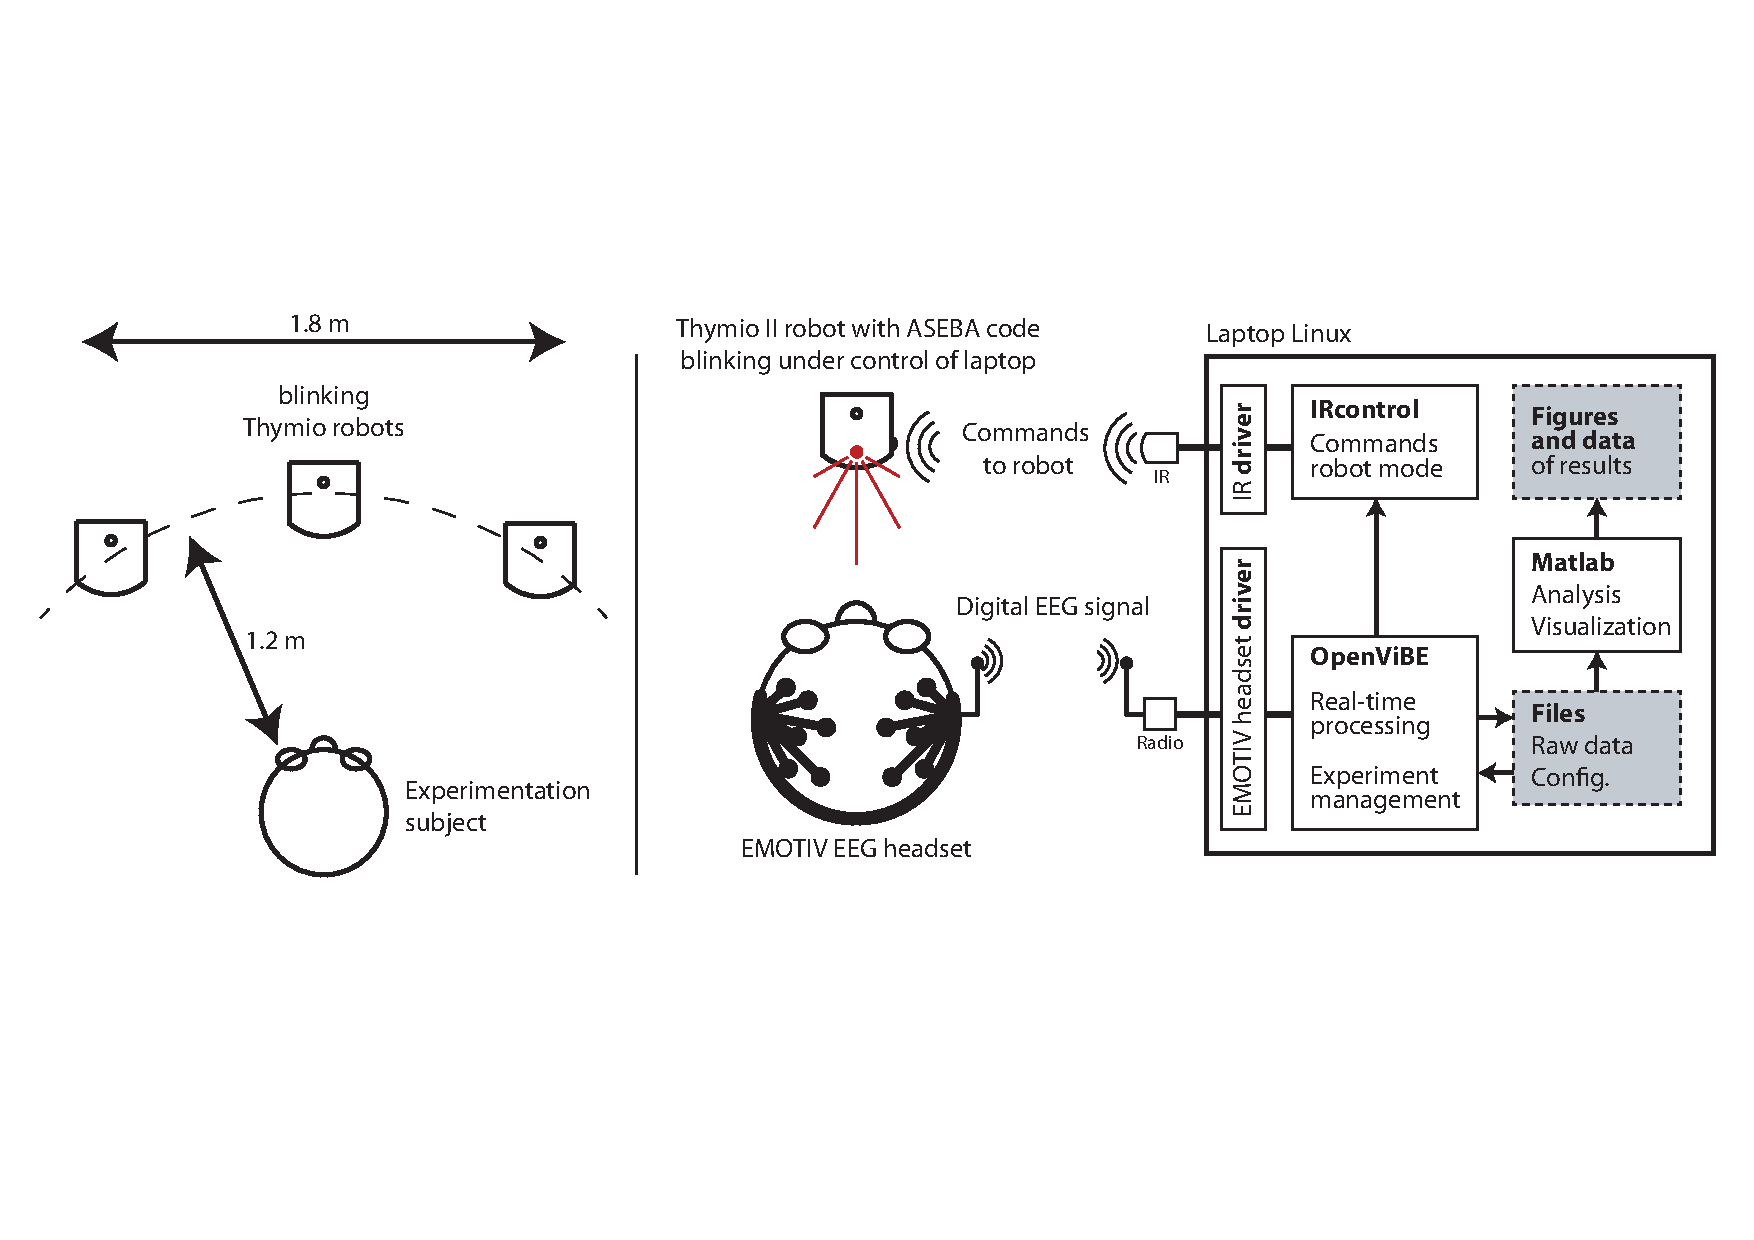
\includegraphics[width=\textwidth]{figures/schema-global.pdf}
\caption{Configuration of the experiment: The left illustrates the spatial arrangement of the experiment; while the right shows the summary of the signal acquisition and processing chain.} \label{fig:thymioinstall}
\end{figure}

\begin{figure}
\center
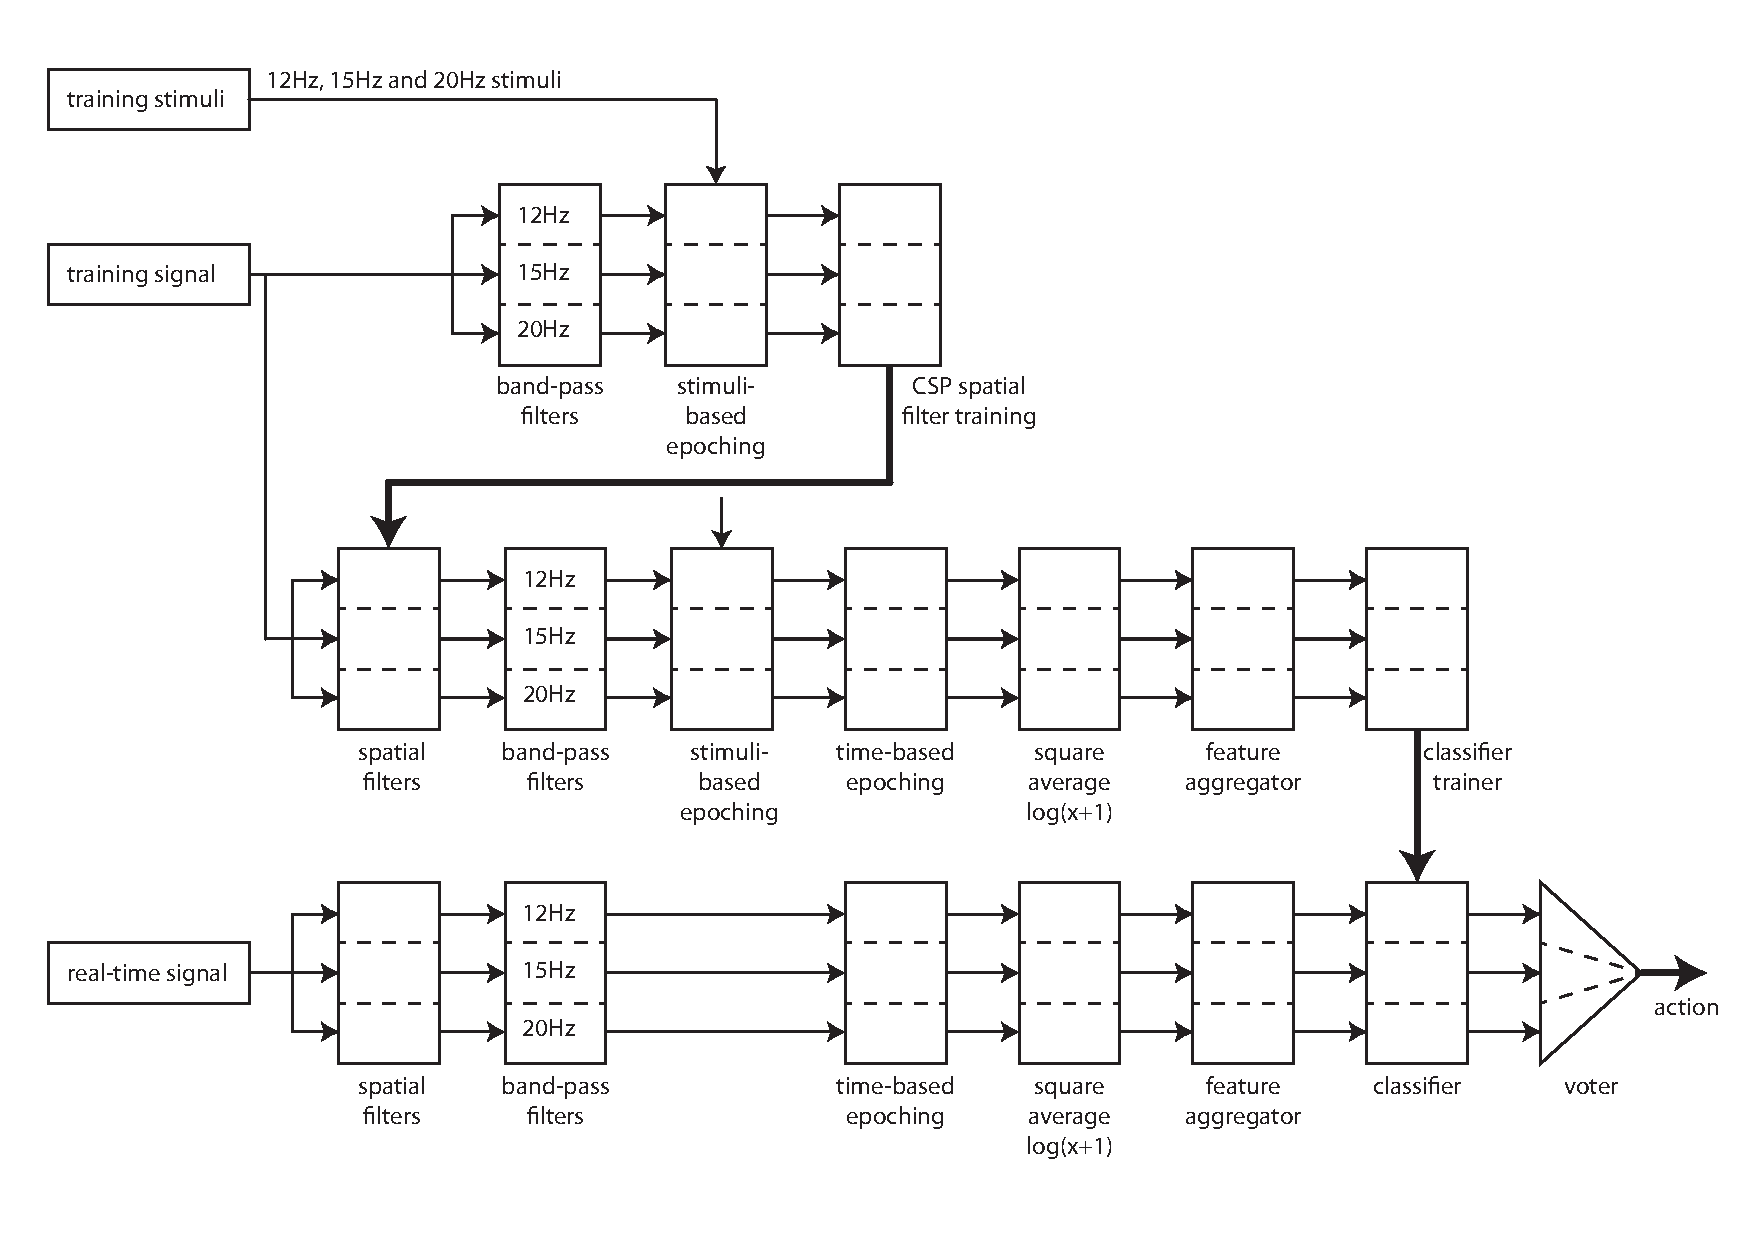
\includegraphics[width=\textwidth]{figures/schema-openvibe.pdf}
\caption{Configuration of the processing chain based on the LDA classifier : The first processing line is used to train the spatial filters, the second to train the classifier, and the third is used to test the whole processing chain.} \label{fig:LDA}
\end{figure}


\subsection{Data analysis}
As illustrated in Figure~\ref{fig:LDA}, the 14-channel EEG data from the Emotiv EPOC is first filtered to focus on 12, 15 and 20$Hz$ using three band pass filters of interval ranges: [11.75, 12.25], [14.75, 15.25] and [19.75, 20.25]. For each frequency, the EEG signals were separated into two groups of 14-reconstructed channels using a common spatial pattern (CSP) filter. Later the multi-variant signals were divided into epochs and the signals in the epoch were squared, averaged and followed by a natural logarithm of the value. These values were used to compute the coefficients for the CSP spatial filters and to train the three LDA classifiers. Each of the classifier classified the epoch vector based on the specific observed blink frequency as target and others as non-targets. For details of the processing chain, please refer to \cite{openvibeSSVEP}. 

\subsection{Results and discussions}
For each of the four sessions we carefully studied the CSP filter output. In our experiments we are analyzing SSVEP signals, therefore, we expected to see large values in regions: P7, O1, O2 and P8 because these provide information about the electrical activity in the occipital lobe. However, we found unpredictable and inconsistent distribution of weights in this region of the brain. In sessions 1 and 2, some importance seems to be given to this part of the brain which would demonstrate some success; however the finding does not hold in sessions 3 and 4. Further analysis shows that the positive responses of the occipital zone as highlighted in sessions 1 and 2 was originated under no blinking condition. In addition, the CSP algorithm sometimes gave great importance to AF4 electrodes and F3 which are frontal electrodes known for the low quality of their signal and their powerful muscle artifacts. Figure \ref{fig: CSP_20} illustrates an example where the CSP filter has attributed low importance to EEG channels in the occipital region known to be neurologically important in the SSVEP process while high importance has been given to noisy and less relevant locations. This malfunctioning of the training process is probably due to the lower quality of the signals acquired by the EEG. As a result, the overall algorithm generated very poor results with a recognition rate close to random.\\
\\
\begin{figure}
\center
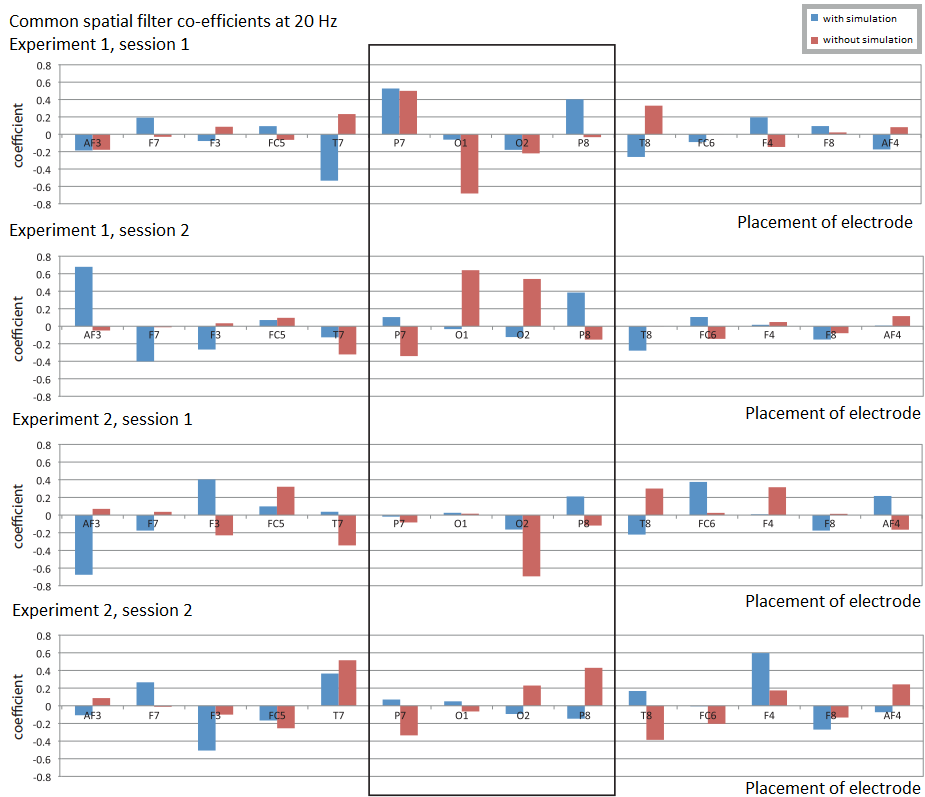
\includegraphics[width = \textwidth] {figures/Untitled_2.png}
\caption{Weights or parameters calculated by the CSP algorithm on the 20$Hz$ signals for four sessions. The captions on the X-axis follow the international code of EEG headset electrode location.} \label{fig: CSP_20}
\end{figure}
\\
Based on our experience with the LDA-based classifier, we realized that our setup with the the Emotiv device and the Thymio has a lot of parameters that require careful attention. For example: the choice of effective frequency range, LED color and the range of effective distance between the user and the robot. Firstly, the Thymio's LEDs have a refreshing rate of 243.75$Hz$, whereas most screen's refreshing rate is around 60$Hz$. Therefore at low frequencies, one must pay attention to choose divisors of the refreshing rate as the blinking frequency to avoid blinking irregularities perceivable by the human eye. This greatly restricts the choice of the effective frequency range. As the refreshing rate grows this factor becomes negligible and the frequencies can be chosen more conveniently. Furthermore, compared to most SSVEP scenarios where researchers either used screens or plain white lights as visual stimulus this set-up uses robots and RGB LEDs. Most importantly, the robot-based setup raises the question of moving targets: How does the variation in distance between the user and the targets impact the EEG signal? Answers to these question are crucial, as moving robots will certainly be at varying distances from the user.\\

\section{Study 2: Robot selection using CCA-based SSVEP classifier}
\label{sec:CCA_approach}
In this section, we studied the impact of three important stimulus parameters: blinking frequency, blinking color and distance to the stimulus. These studies not only make sense within the context of our study but also have scientific interest. To our knowledge there has not been any study featuring the range of these stimulus parameters considering the Emotiv EPOC EEG device. We know from literature that the recognition reliability decreases if either frequency or the distance to stimulus target increase \cite{herrmann2001, wu2013effect}. Moreover, we know that the white color can emit three times as much light as red, green or blue; and stimulates all three cone cells in the eye which could potentially lead to stronger neural responses \cite{aljshamee2016discriminate}. However, the characteristic details for this particular headset is unknown. Given the reduced signal acquisitive capability of Emotiv EPOC device as compared to standard medical grade EEG headsets; we expect the limits to be significantly lower.\\
\\
This section highlights three short studies featuring parameter tuning (frequency, distance to the stimuli and LED color). The outcome of these individual studies in taken into account to design and propose the robot selection methodology. Furthermore, we explain the experimental setup and the data-collection protocol. The CCA can be thought of as a generalization of the correlation measure to multivariate signals. This particular algorithm was chosen because Lin et al. achieved good results with the same headset by using CCA to address SSVEP classification \cite{Lin2014}. The principle of this approach is as follows: given $X$, $Y$ are two multivariate signals, the optimisation problem of CCA is finding $\rho$ such that
\\
\begin{equation}
\label{rho}
\rho = \max_{a, b \in \mathbb R^n}  r_{ a^\top X, b^\top Y}
\end{equation}
Here,  $r_{XY}$ is the correlation between $X$ and $Y$,  $a$ is the eigenvector associated to the largest eigenvalue of $S(X, X)^{-1} S(X,Y) S(Y, Y)^{-1} S(Y, X)$, and $b$ is the eigenvector associated to the largest eigenvalue of $S(Y, Y)^{-1} S(Y, X) S(X, X)^{-1} S(X, Y)$, where $S(X, Y)$ is the covariance matrix. The proof  can be found in \cite{rencher2003}.

\subsection{Experimental setup, data collection and analysis}
The short experiments for parameter tuning were similar to the experiment conducted in section \ref{sec:ML_approach}. However for each parameter, the experiments were conducted on different subjects. The experiments consisted of multiple trails; where each trail was 7$s$ long with breaks of 3$s$. For each parameter the corresponding frequency spectrum was calculated using fast Fourier transform. To quantify the detectability of the SSVEP we defined the recognition ratio. Given a particular frequency $f$, let $F$ and $R$ be two disjoint subsets of the averaged spectrum such that $F$ contains the spectrum of the frequencies $[f-1, f+1]$, and $R$ contains the frequency range $[6, f-1[ \,\cup\, ]f+1, 18]$. The recognition ratio $q$ is defined as:
\begin{equation}
\label{recog_rat}
q =:\frac{\max F}{\max R}
\end{equation}
\\
The recognition ratio provides the ratio of the highest peak within $[f-1, f+1]$ to the highest peak in the rest of the spectrum. The neural response to a regularly blinking stimulation, called SSVEP, is characterized by a peak in the spectrum of the signal at the same frequency as the blinking frequency. Thus, if the recognition ratio is above 1, then the highest peak is within $1\,\mathit{Hz}$ of $f$, and the SSVEP can be considered detectable. 
Otherwise, the SSVEP cannot be observed. 
Please note that we decided to consider peaks up to $1\,\mathit{Hz}$ off from the stimulation frequency as valid SSVEP responses because we always have at least $2\,\mathit{Hz}$ difference between one stimulation frequency and the another. This band could be restricted, as further analysis of my results has shown that neural responses are in general very accurate.

\subsection{Parameter: Stimulation frequency}
Six frequencies were tested (9, 12, 15, 18, 21, and 24$Hz$). For each frequency condition, five trials were performed on three different subjects. The blinking light was set 1$m$ away from the subject. Figure \ref{fig:graph-frequences} confirms the decrease in the amplitude of the neural response as the frequency grows as already described by \cite{herrmann2001}; furthermore it shows that the detection fails beyond 15$Hz$. Therefore, we can conjecture that SSVEP activity can be measured with this headset, provided low frequencies are chosen. Based on these observations, we restricted the frequency band in the following two studies; the chosen interval: $[7\,\mathit{Hz}, 17\,\mathit{Hz}]$.

\begin{figure}
\center
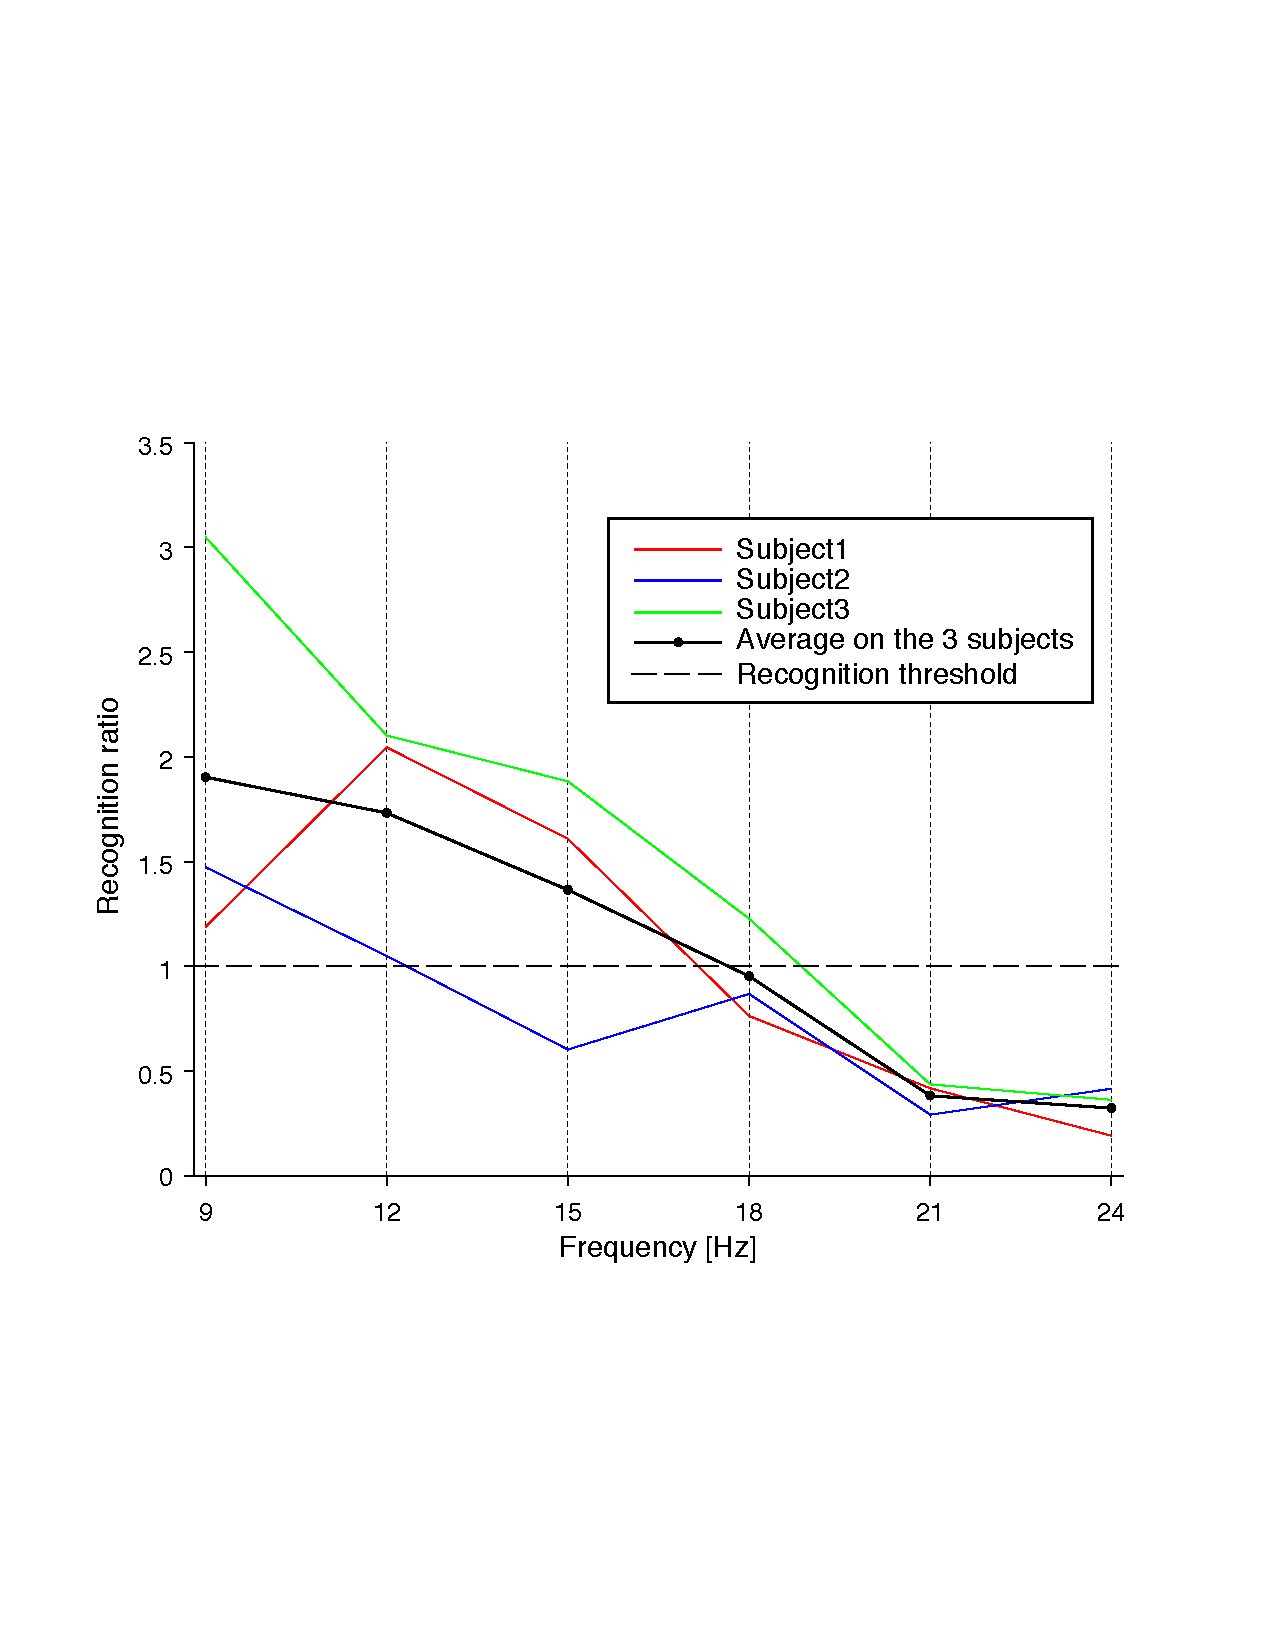
\includegraphics[width=0.8\textwidth]{figures/graph-frequences.pdf}
\caption{Recognition of a red visual stimulus in the EEG spectrum based on its blinking frequency. Each of the three subjects has been subjected to five trails for each frequency; the trail period is 7$s$. The plotted recognition ratio for each frequency represents the values of the averaged power spectrum of the five stimulation trails.} \label{fig:graph-frequences}
\end{figure}

\subsection{Parameter: Stimuli distance}
As a second parameter, we analyzed the impact of varying distance between the EEG user and the blinking target robots; considering each of the frequencies: 7, 9, 12, 15, and 17$Hz$; the tested distances were: 30$cm$, 1$m$ and 2$m$. The experiment was conducted on three subjects; where each subject performed four. Figure \ref{fig:graph-distances} summarizes the result; there is not much difference in neural response between 30$cm$ and 1$m$, however the response starts to deteriorate at 2$m$. Indeed, the recognition ratio at 2$m$ falls under 1.0 at 13$Hz$. The reasons are: (1) target becomes smaller with increasing distance and (2) the EEG signal and LED light strength deteriorates.

\begin{figure}
\center
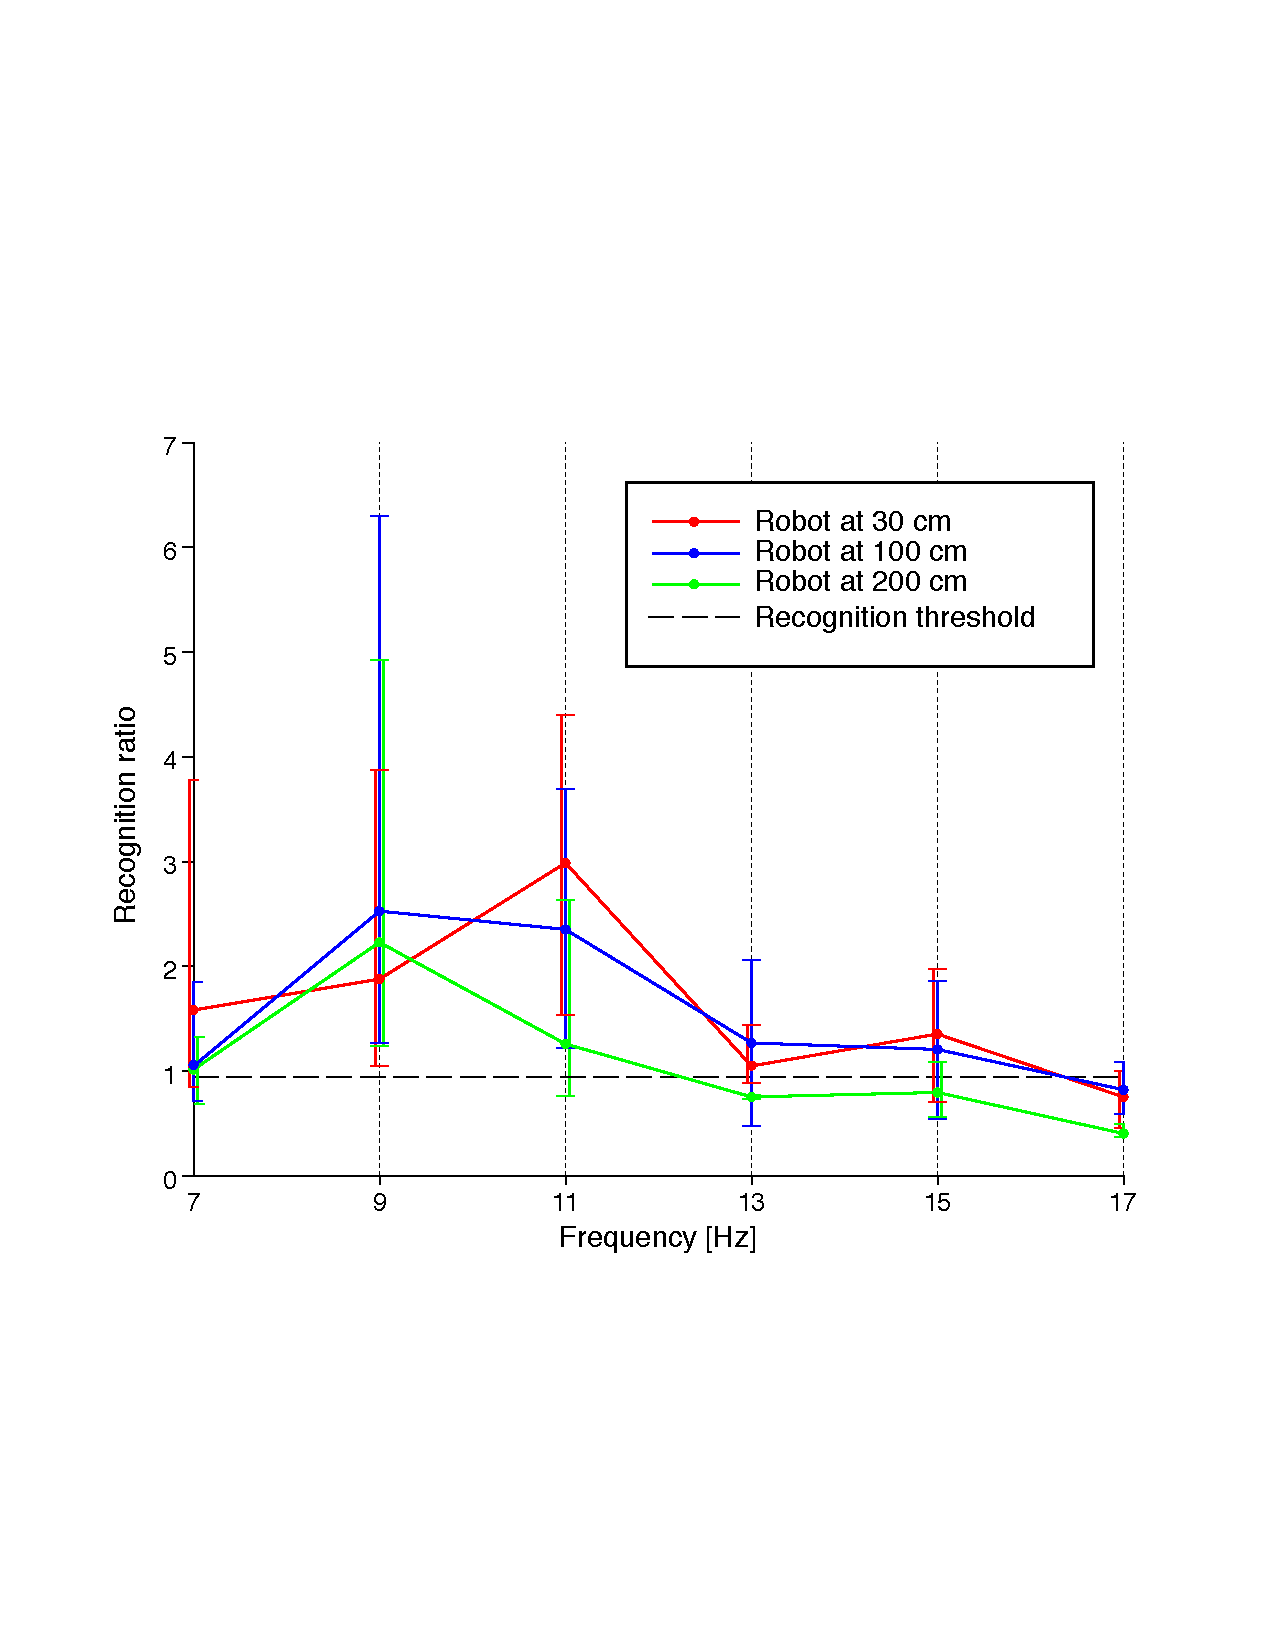
\includegraphics[width=0.8\textwidth]{figures/graph-distances.pdf}
\caption{Recognition of a red visual stimulus in the EEG spectrum based on the distance of the robot. Four trails per subject for each distance and frequency combination was performed. The plotted recognition ratio for each frequency and distance combination represent the values of the averaged power spectrum of all the stimulation trails on all the subjects.}
\label{fig:graph-distances}
\end{figure}

\subsection{Parameter: Stimulation color}
The study featuring stimulus color was similar to the stimulus-distance experiment. Four trials were conducted for each combination of frequency (7, 9, 12, 15, and 17$Hz$) and LED color (red, green and white). The target robot was at 1$m$ from the subjects. Figure \ref{fig:graph-couleurs} show that the best results were obtained using the red or green colors; it is clear that white does not increase the neural response. Although, the neurological reasons behind such observation is unclear; this finding is certainly in line with other similar findings in literature.

\begin{figure}
\center
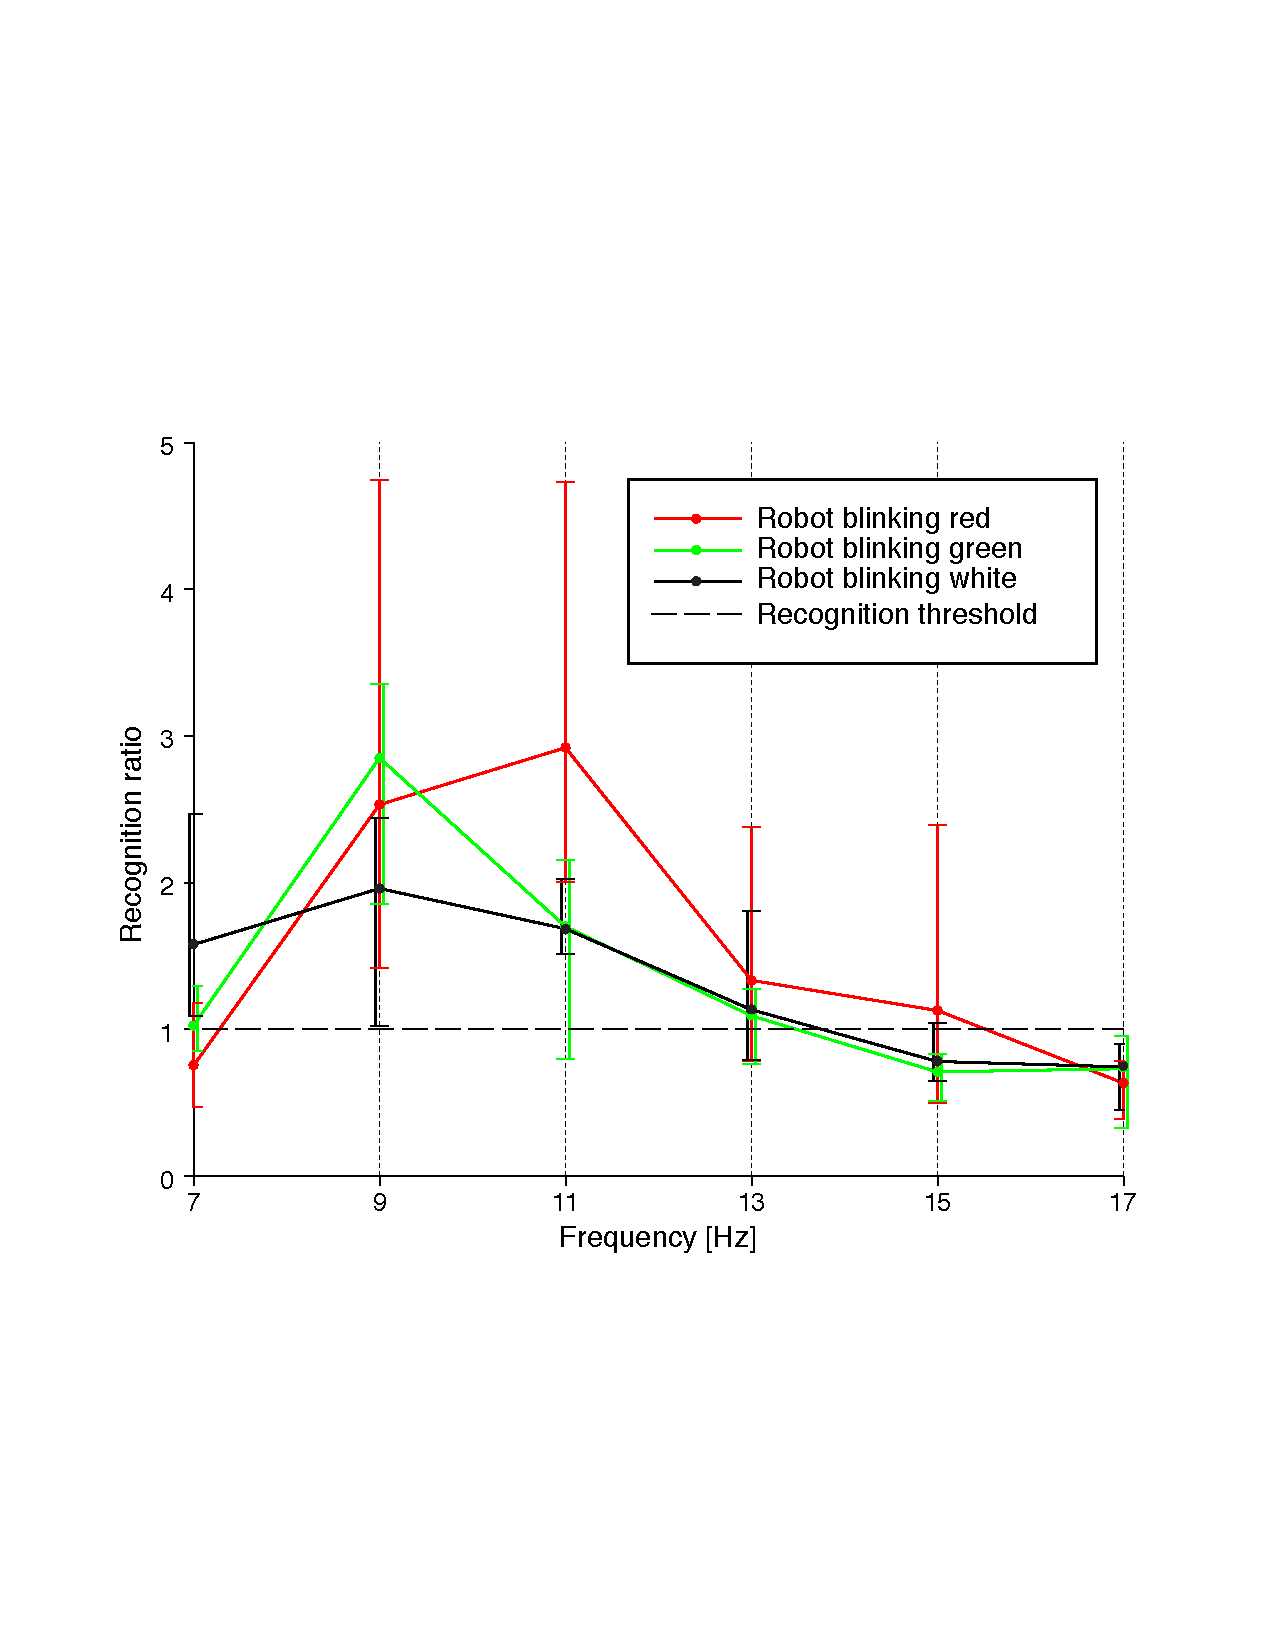
\includegraphics[width=0.5\textwidth]{figures/graph-couleurs.pdf}
\caption{Recognition of a visual stimulus in the EEG spectrum based on its color. Four trails per subject for each color and frequency combination was performed. The plotted recognition ratio for each frequency and distance combination represent the values of the averaged power spectrum of all the stimulation trails on all the subjects.} \label{fig:graph-couleurs}
\end{figure}

\subsection{Robot selection methodology using CCA-based SSVEP analysis}
\subsubsection{Experimental setup and data collection}
Based on the results from the short studies, we designed an experiment to implement and test the robot selection methodology using CCA-based SSVEP analysis. The schematics of this setup can be found in figure \ref{fig:experiment-set-up}. Three Thymios blinking in red at frequencies of 8, 10 and 12$Hz$ were placed in a half circle, 90 degrees apart. The user was equipped with an IR remote control and had his/her EEG signal analyzed in real-time using the CCA algorithm. When the user looked at the robot he/she wanted to control, the EEG signals were acquired from the Emotiv device and a prediction was made by the processing chain, this information was transmitted via IR to the robots. The selected robot would turn green and execute the command received from the IR remote control while the other robots would remain red and ignore these commands. The user was exposed to 15 trails of 15$s$ each: 5 trails at each frequency. Before each trail, the subjects were told which of the three robots he/she should look at and was given 4$s$ to prepare. During the trail, the subject had to concentrate on one robot even though all three robots were blinking; 3$s$ break followed each trail. To assess the reliability of this methodology, the experiment was conducted on 10 different subjects. The subjects were aged between 17 and 48: three women (age: 17, 32 and 44) and seven men (age: 18, 18, 19, 29, 35, 37, 48). 

\begin{figure}
\center
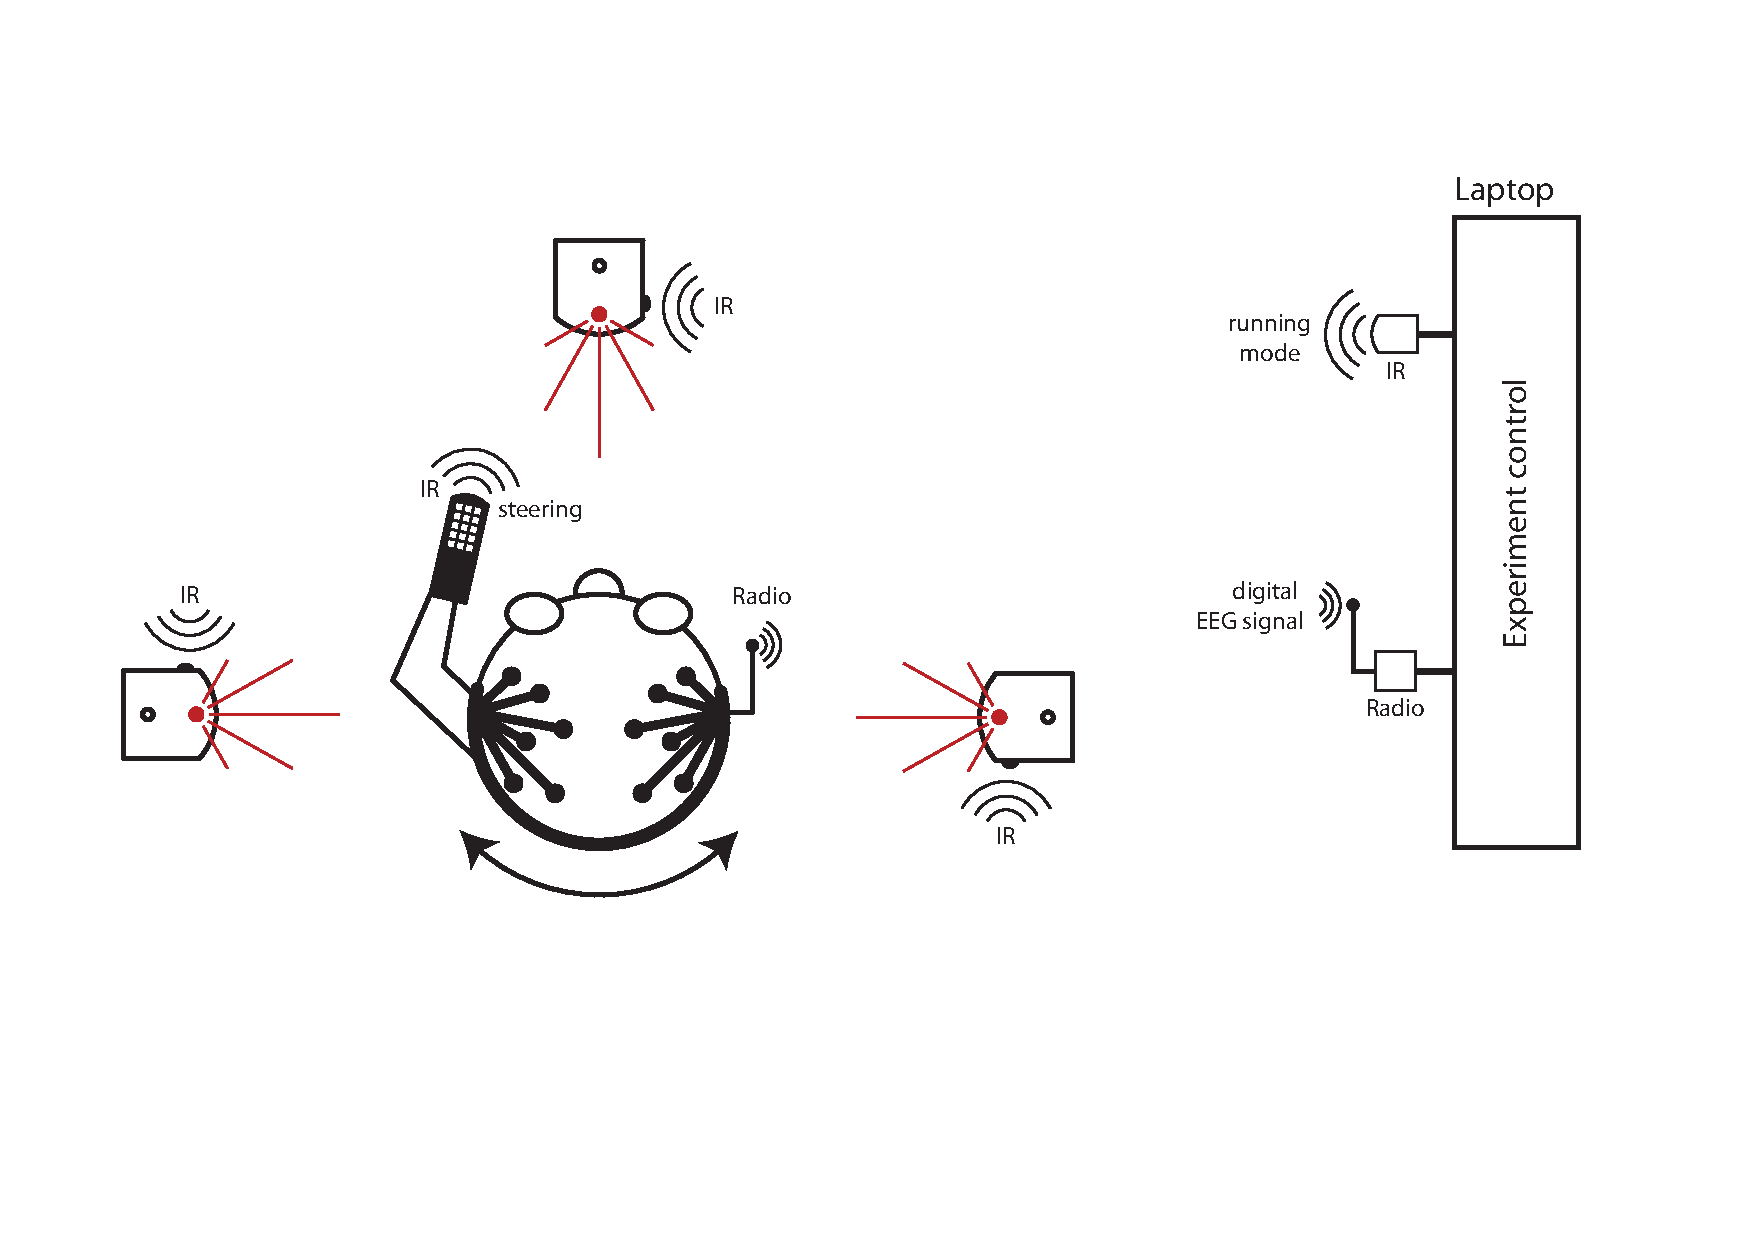
\includegraphics[width=0.6\textwidth]{figures/schema-global2.pdf}
\caption{Setup of the experiment, showing the configuration of the user with respect to the robots and the communication channels used for interaction. The details schematics of the computational unit: signal acquisition and processing chain is the same as shown in figure \ref{fig:thymioinstall}} \label{fig:experiment-set-up}
\end{figure}

\subsubsection{Data analysis processing chain}
Figure \ref{fig:schema-openvibe-cca} shows the details of the processing chain. The predominant SSVEP EEG signal from the occipital region of the brain was acquired and stored in 8 second buffer. At each iteration the signal length parameter of the trimming function was changed. Initially, this parameter is set to 2$s$, so the last 2$s$ of the buffered signal was considered. At each iteration, the signal length is incremented by 0.25$s$. This particular signal is correlated to 3 different simulated signals using CCA. These simulated multivariate signals composed of sine, cosine and their first harmonic at the same frequency as the associated stimulus frequency. Later, a voting scheme selects the frequency with the highest correlation as the new predicted stimulation frequency. For the loop to end successfully, four consecutive predictions must coincide. If the signal length reaches 8 secs, the loop was stopped and no prediction was made.

\begin{figure}
\center
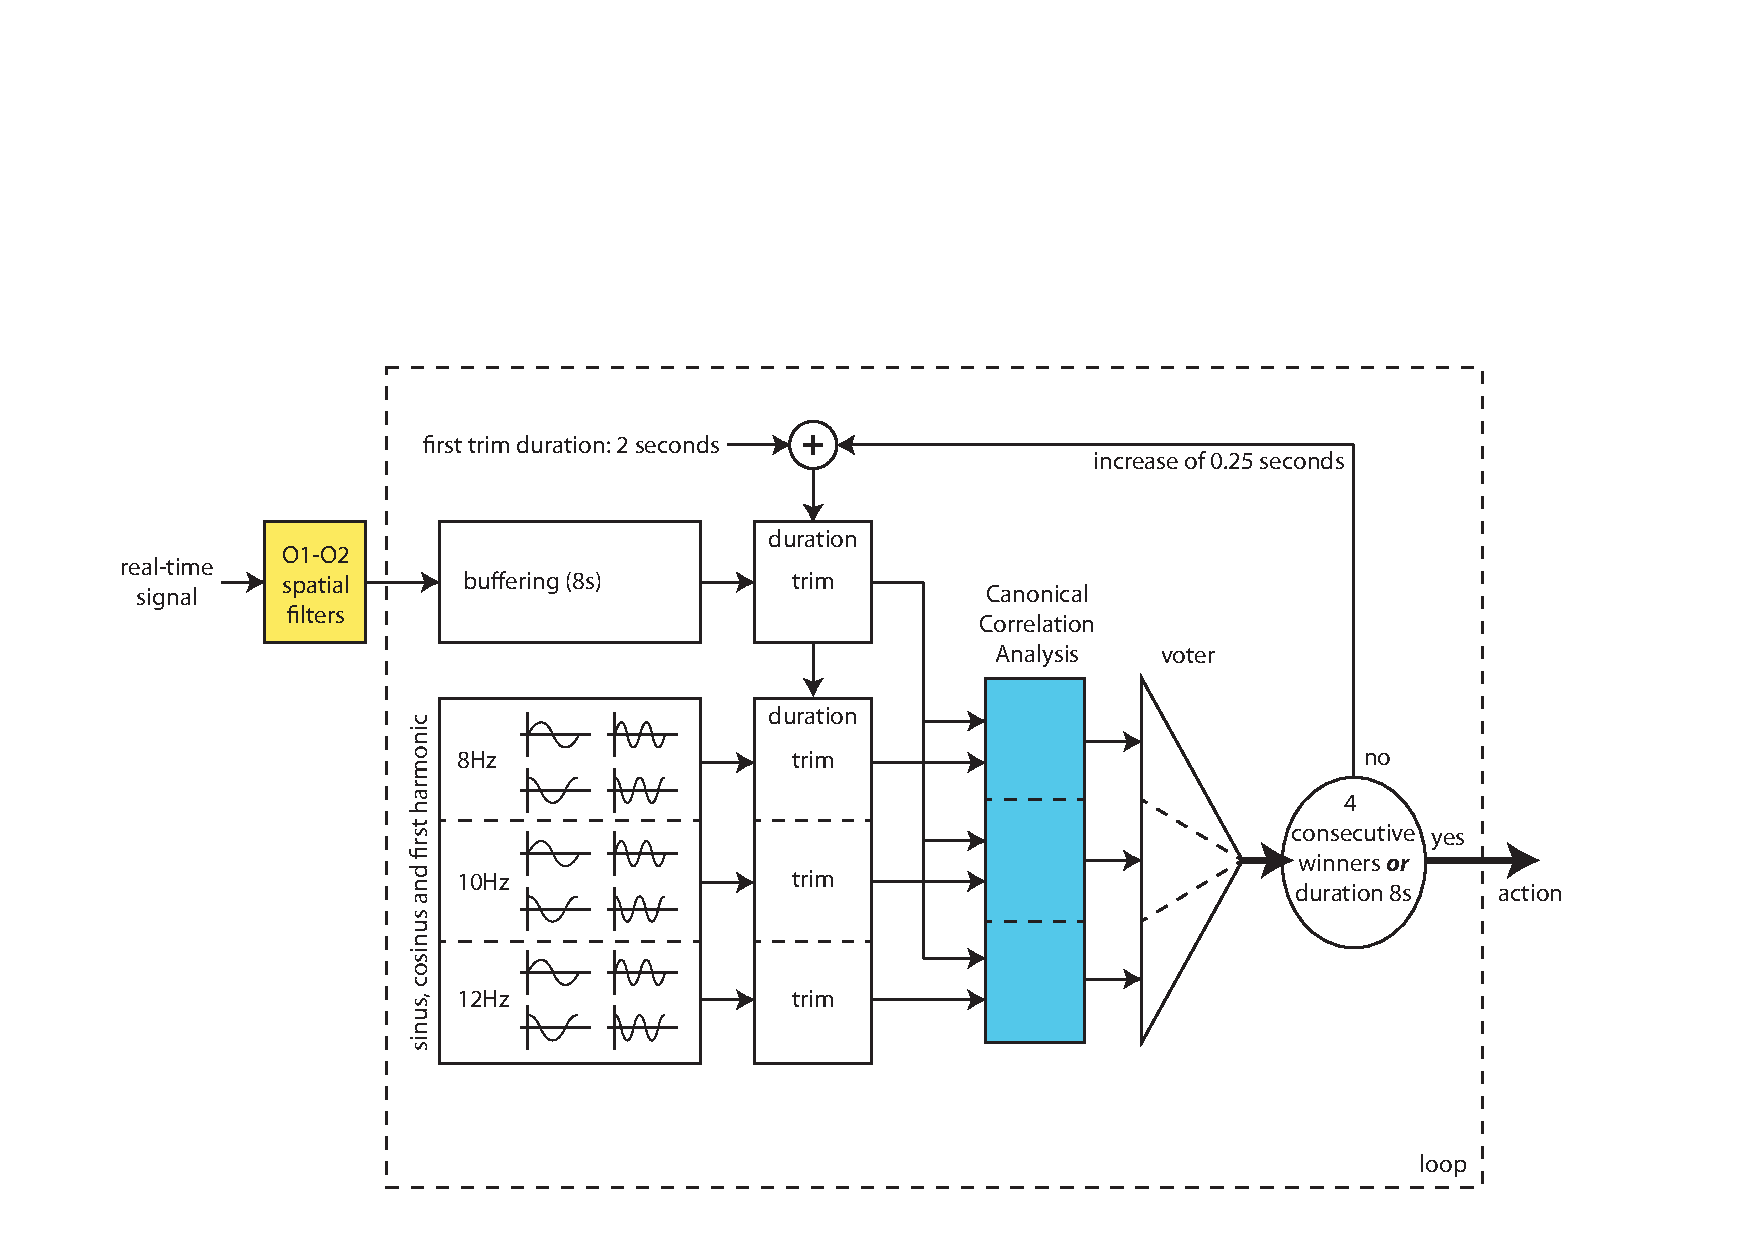
\includegraphics[width=0.7\textwidth]{figures/schema-openvibe-cca.pdf}
\caption{Signal processing chain used the occipital signal O1 and O2. These signal are first buffered; only the last part of the buffer is used for processing. The length of this period is variable and increased at each processing loop. The signal is compared with ideal signals and the best fit is selected. Four consecutive coinciding predictions are required to have a final selection. The loop is terminated when the whole buffer of 8 secs has been used}
\label{fig:schema-openvibe-cca}
\end{figure}

\subsubsection{Results and discussions}
Figure \ref{fig:all_time_reconn} shows the recognition rate as function of time; the data presented was averaged over all predictions made on all 10 subjects in all stimulations. It can be seen that the recognition rate starts randomly and increases gradually to plateau around 75\%. The similar increase in recognition reliability after 4$s$ can also be seen in figure \ref{fig:taux-reconn}; this graph shows the average recognition rate per frequency. We can observe that the lowest reliability is at 12$Hz$; while the highest is at 10$Hz$ with very little standard deviation. The variance between the subjects can be observed in more detail in figure \ref{fig:all-results-reconn}; these graphs show the average recognition rates per subject per frequency. The reliability of 10$Hz$ can be seen in different subjects but especially in subjects 5 and 7; where the recognition rate at 10$Hz$ is double compared to 12$Hz$. Lastly, this graph also shows the divergences between different people: subject 1 has a 98\% recognition rate at 8 Hz while subject 5 is around 40\% for the same frequency. This is a key characteristic of EEG that makes EEG analysis so delicate and must be carefully considered when developing new applications.

\begin{figure}
\center
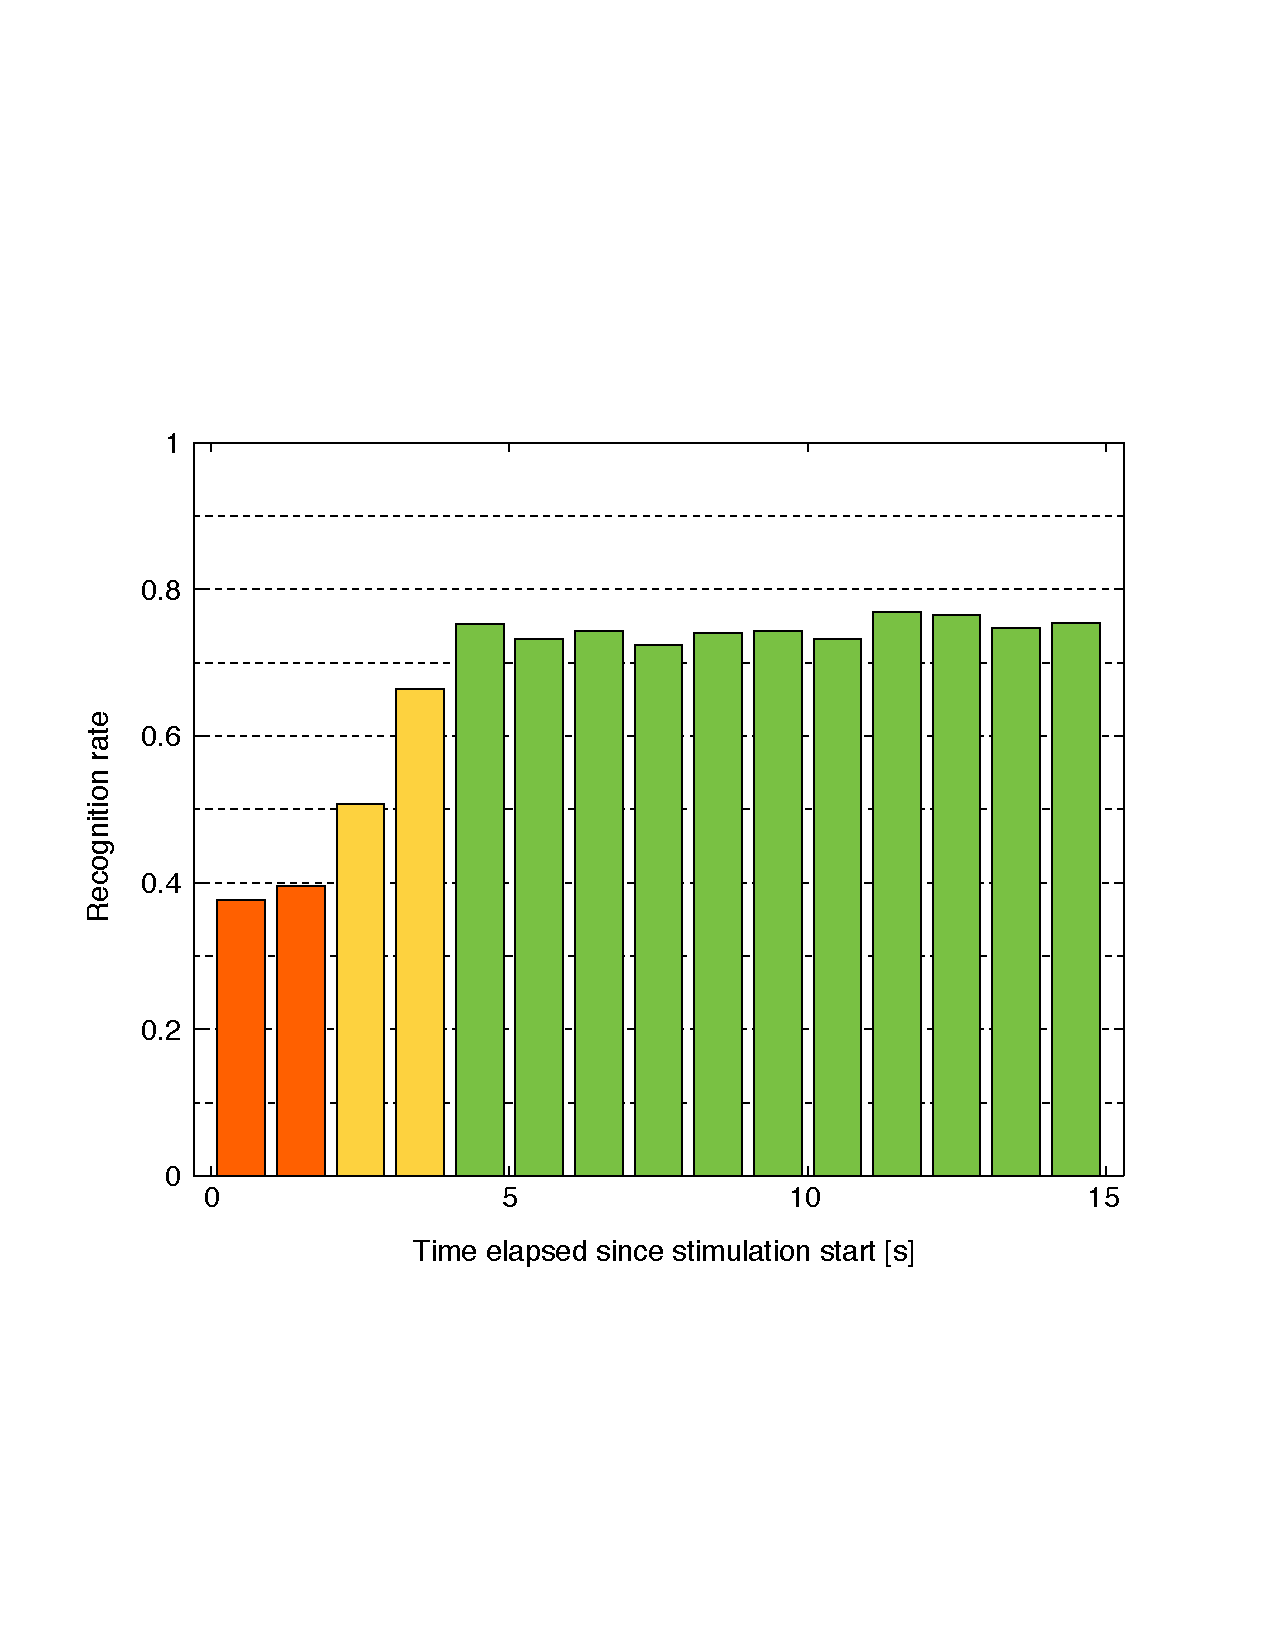
\includegraphics[width=0.5\textwidth]{figures/all_time_reconn.pdf}
\caption{Frequency recognition rate versus time during the 15 secs of stimulation. These numbers are an average over 10 subjects considering the 5 trails of $15\,s$ each and the stimulation frequencies (8, 10 and 12 Hz).} \label{fig:all_time_reconn}
\end{figure}

\begin{figure}
\center
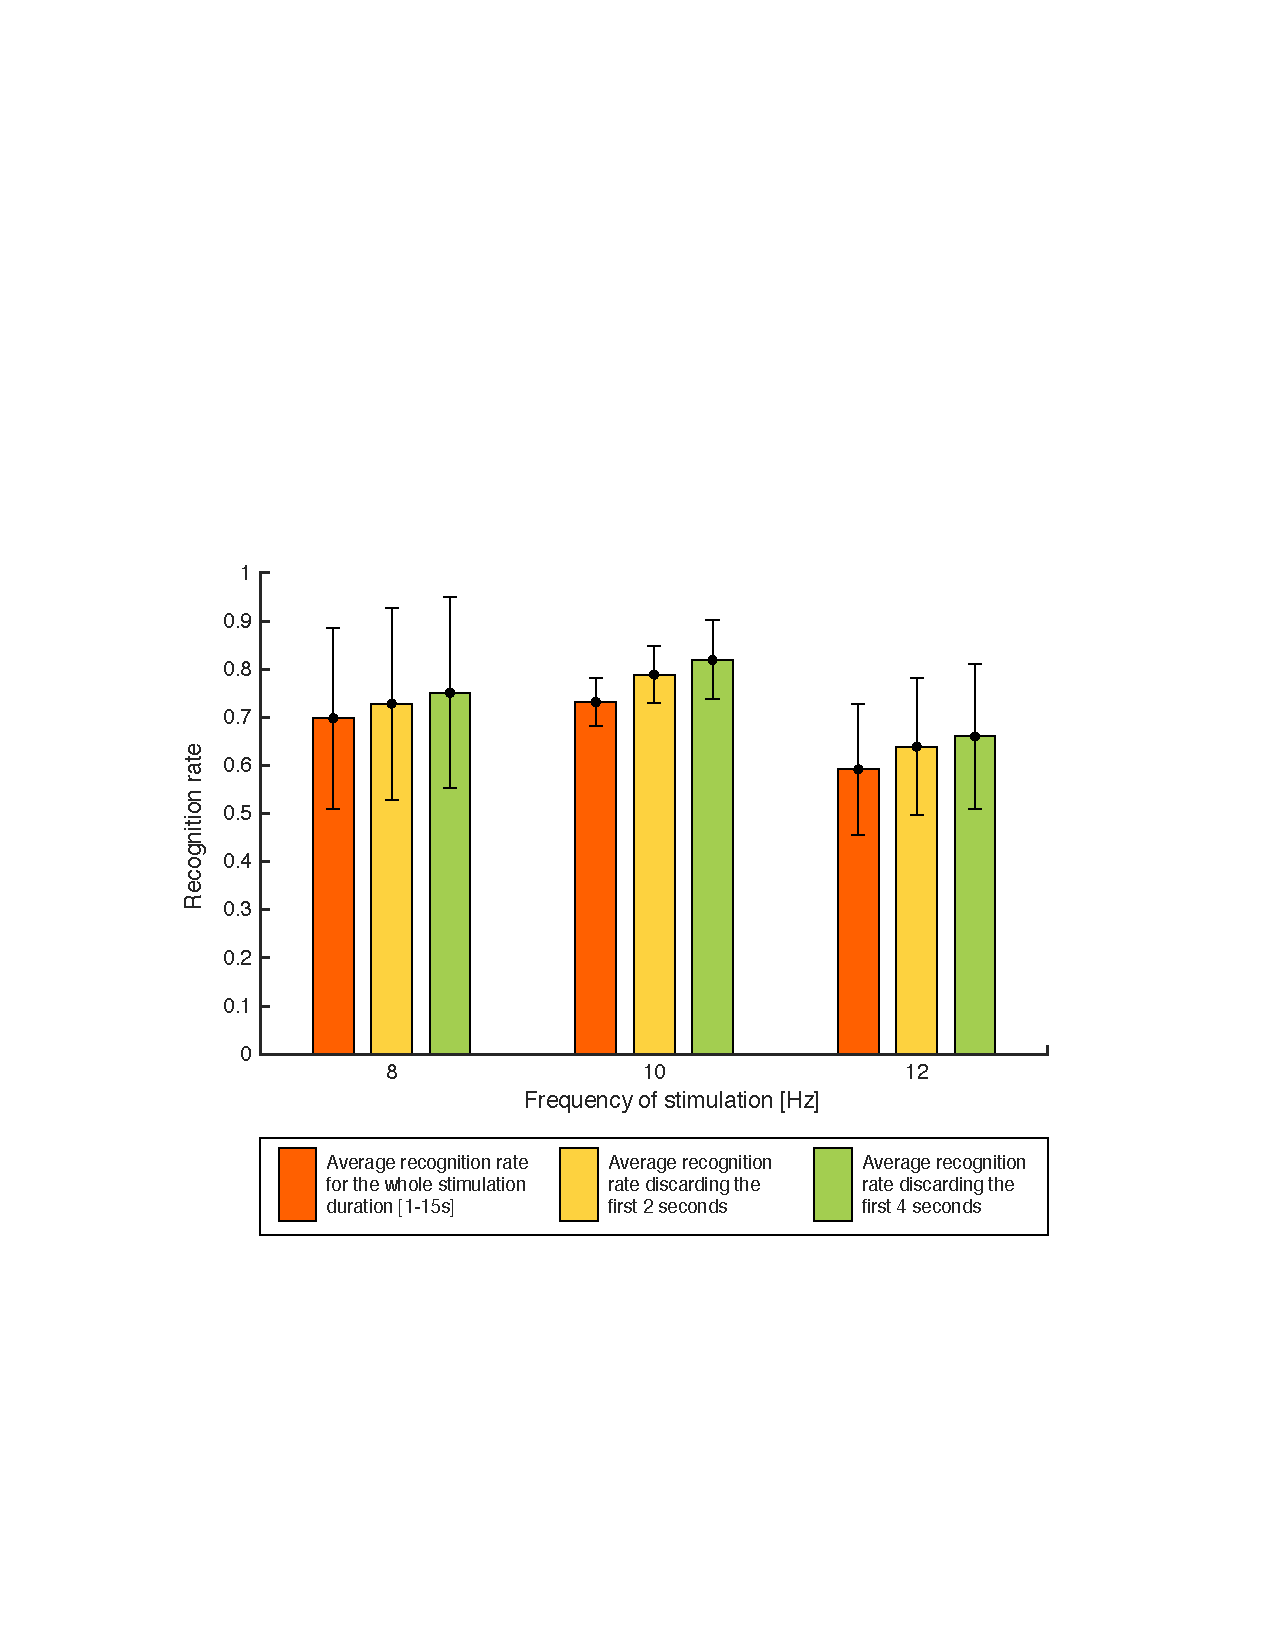
\includegraphics[width=0.5\textwidth]{figures/taux-reconn.pdf}
\caption{Frequency recognition rate per stimulation frequency and per delay between start of stimulation and start of recognition process. These numbers are an average over 10 subjects considering the 5 trails of $15\,s$ each and the stimulation frequencies (8, 10 and 12 Hz). The figures for each subject are detailed in figure \ref{fig:all-results-reconn}.}
\label{fig:taux-reconn}
\end{figure}

\begin{figure}
\center
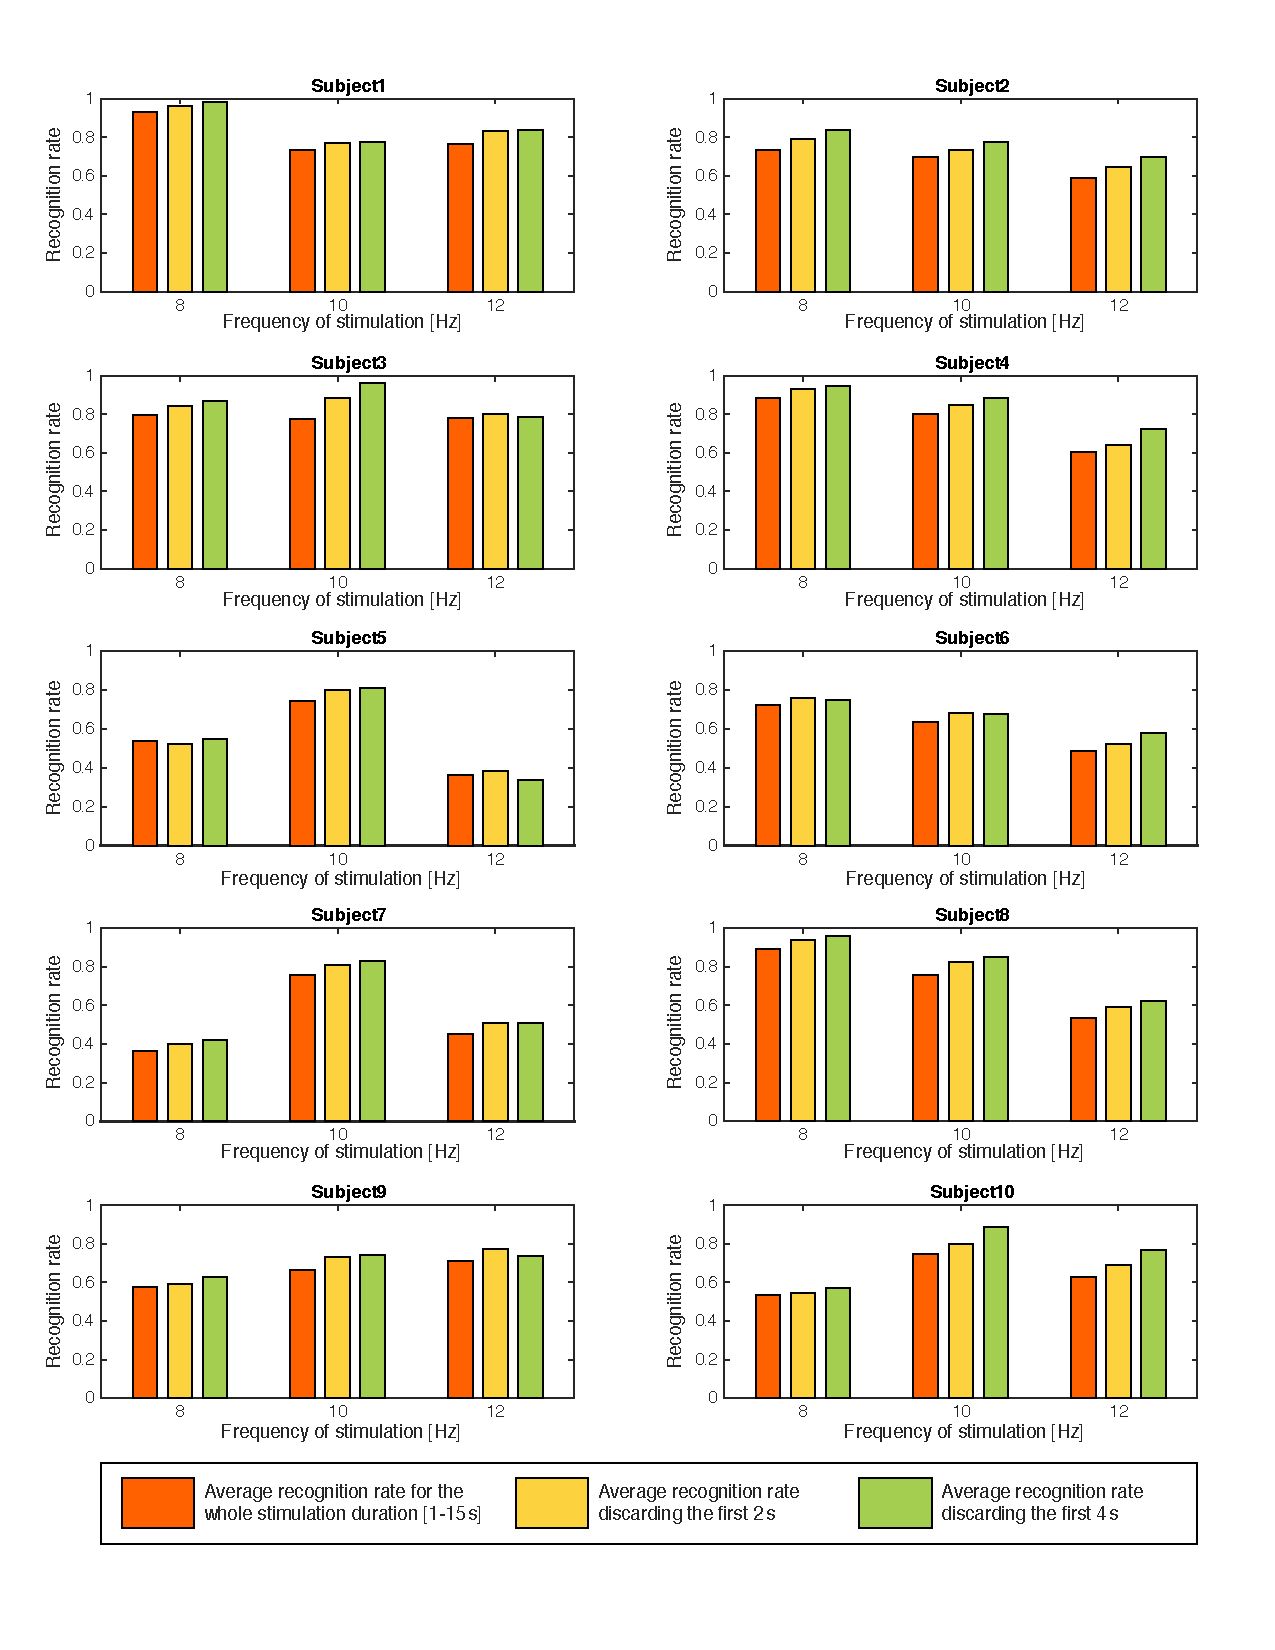
\includegraphics[width=0.7\textwidth]{figures/all-results-reconn.pdf}
\caption{Frequency recognition rate per subject and per stimulation frequency, considering the different stimulation durations.}
\label{fig:all-results-reconn}
\end{figure}

Based on the results, we can observe that the time required to recognize and select the robot is at least 4 seconds. Based on the algorithm the best result that we can get is after 3 seconds, this matches with the results achieved in literature. Although this signal processing chain does not require a training session as opposed to systems that use machine learning algorithms; this delay of 4$s$ is a clear drawback to this prediction system. Moreover, the stability of this set-up is remarkable: it shows that despite the numerous artifacts, it is possible to guarantee, on average, a recognition rate of 75\% at any time after the first $4\,s$. The small variation also suggests that the prediction system used, as it is, will not provide better results. 

\section{Conclusions}
This study systematically analyzes two state-of-the-art SSVEP-related EEG classification techniques and some of their key parameters for tackling the robot selection problem using the Emotiv EPOC, and proposes a new methodology for addressing human-swarm interactions. 
In respect to the existing literature based on gesture or vice commands, this approach is more intuitive, being based only on the gaze of the user. 
In respect to other potential gaze-based approaches, such as eye-tracking devices, the CCA-based SSVEP classifier does not need training nor calibration, still reaching performances that in some individuals can reach success rates well above 75\%.

This is also the first study giving an estimation of the potential distance of robot detection using this technique.
Despite the limited range observed in our experiments, that is less than 2$m$, this distance has to be considered in respect to the size of the robot and the type of visual stimuli.
In this project, the stimuli comes from two LEDs placed in the body of a 10$cm$ large robot. 
We can speculate that a larger and more visually salient robot could be selected at a much higher distance, making a real application possible.


Another limitation comes from the number of available frequencies.
Despite the possibility to classify a very high number of very close frequencies \cite{SSVEPfiability}, the number of possible detected robots stays finite, limiting the scalability of the approach. 
However, this selection technique could be combined with other approaches, sur as detection of head orientation, allowing to pre-select part of the swarm and use this technique for a subset of the swarm.


Finally, some factors that are uncontrollable in a real world applications, such as muscular artifacts or personal attitudes of the pilot, could impact negatively the performances of such a solution.
Other factors, such as the relative surrounding brightness, the variable distance to the targets, and the blinking light interferences with other robots should be carefully considered to reach the best performance.


To conclude we believe, despite the limiting factors highlighted by our work, that the very positive results show that an efficient combination of EEG and swarm-robotics could open new interesting possibilities in human-swarm interactions.\\

%	Finally, while some factors that are uncontrollable in a real world application, such as muscular artifacts; the relative surrounding brightness, variable distance to the targets and blinking light interferences from other robots must still be controlled; 

\begin{acknowledgement}
Many thanks to Dr. Ricardo Chavarriaga, Dr. Claire Braboszcz and Dr. Serafeim Perdikis for the constructive discussions about experiments involving EEG, and to Dr. J\'er\^ome Scherer and Prof. Marco Picasso for their help on mathematical issues in the signal processing. This work was partially supported by the Swiss National Center of Competence in Research "Robotics".
\end{acknowledgement}

\bibliography{mybib}


\end{document}
